\section{Experiments}

\begin{table*}[!t]
\begin{center}
\small
\tabcolsep=0.015\linewidth
\resizebox{\linewidth}{!}{
\begin{tabular}{lcccccc}
\toprule
\textbf{Model Name} & \textbf{Best Exist Rate} & \textbf{Correct Exist Rate} & \textbf{Score} & \textbf{\makecell{Search Attempt\\Valid (\%)}} & \textbf{\makecell{Action Attempt\\Valid (\%)}} & \textbf{\makecell{Preference Elicited (\%)\\(Active / Passive)}} \\
\midrule
GPT-4o & 0.204 & \textbf{0.361} & \textbf{0.329} & 82.48 & 27.82 & 27.32 (24.06 / 3.26) \\
Gemini-2.5-Pro & 0.245 & 0.328 & 0.317 & 77.40 & 29.26 & 29.71 (23.85 / 5.85) \\
Claude-4-Sonnet & \textbf{0.260} & 0.318 & 0.307 & 74.28 & 24.26 & \textbf{34.25} (\textbf{26.31} / 7.94) \\
Deepseek-V3 & 0.148 & 0.218 & 0.210 & 61.22 & 23.62 & 31.82 (18.90 / 12.92) \\
Qwen3-14B & 0.157 & 0.197 & 0.209 & 70.56 & \textbf{33.71} & 30.07 (15.95 / 14.12) \\
Qwen3-32B & 0.154 & 0.211 & 0.206 & 79.42 & 26.89 & 22.01 (13.04 / 8.96) \\
Llama-3.3-70B & 0.120 & 0.209 & 0.198 & 60.51 & 11.29 & 23.25 (13.05 / 10.20) \\
Qwen3-8B & 0.140 & 0.186 & 0.180 & 68.94 & 23.20 & 28.86 (11.15 / 17.70) \\
GPT-4o-mini & 0.102 & 0.173 & 0.166 & 76.10 & 13.55 & 25.43 (12.91 / 12.52) \\
Llama-3.1-8B & 0.073 & 0.171 & 0.159 & 57.99 & 12.13 & 19.87 (8.09 / 11.78) \\
Gemini-2.5-Flash & 0.047 & 0.080 & 0.125 & \textbf{83.62} & 28.14 & 14.00 (11.15 / 2.86) \\
\bottomrule
\end{tabular}
}
\end{center}
\vspace{-3mm}
\caption{{\gymname} main evaluation results across different models (single-choice setting).}
\label{tab:travelgym_results_onechoice}
\end{table*}


\begin{table*}[!t]
\begin{center}
\small
\tabcolsep=0.015\linewidth
\resizebox{\linewidth}{!}{
\begin{tabular}{lcccccc}
\toprule
\textbf{Model Name} & \textbf{Best Exist Rate} & \textbf{Correct Exist Rate} & \textbf{Score} & \textbf{\makecell{Search Attempt\\Valid (\%)}} & \textbf{\makecell{Action Attempt\\Valid (\%)}} & \textbf{\makecell{Preference Elicited (\%)\\(Active / Passive)}} \\
\midrule
GPT-4o & \textbf{0.652} & \textbf{0.725} & \textbf{0.710} & 85.96 & 37.89 & 15.10 (13.11 / 1.99) \\
Gemini-2.5-Pro & 0.604 & 0.685 & 0.673 & 80.43 & 38.01 & 37.25 (28.80 / 8.46) \\
Claude-4-Sonnet & 0.586 & 0.619 & 0.612 & \textbf{87.94} & \textbf{41.17} & \textbf{42.21} (\textbf{30.67} / 11.54) \\
Qwen3-32B & 0.343 & 0.416 & 0.411 & 82.76 & 34.24 & 17.72 (10.81 / 6.90) \\
Deepseek-V3 & 0.351 & 0.398 & 0.391 & 61.91 & 21.06 & 16.96 (10.18 / 6.78) \\
Llama-3.3-70B & 0.294 & 0.366 & 0.372 & 63.46 & 21.72 & 31.72 (16.68 / 15.04) \\
Gemini-2.5-Flash & 0.279 & 0.316 & 0.311 & 84.27 & 33.58 & 15.32 (11.67 / 3.64) \\
GPT-4o-mini & 0.227 & 0.294 & 0.283 & 81.54 & 24.90 & 20.18 (10.46 / 9.72) \\
Qwen3-14B & 0.204 & 0.249 & 0.258 & 71.48 & 35.06 & 26.21 (13.07 / 13.14) \\
Llama-3.1-8B & 0.117 & 0.252 & 0.234 & 61.38 & 12.20 & 26.01 (7.80 / 18.20) \\
Qwen3-8B & 0.147 & 0.186 & 0.182 & 69.83 & 23.26 & 20.31 (7.95 / 12.37) \\
\bottomrule
\end{tabular}
}
\end{center}
\vspace{-3mm}
\caption{{\gymname} main evaluation results across different models (multi-choice setting).}
\label{tab:travelgym_results_multichoice}
\end{table*}



\subsection{Settings}
\paragraph{Gym Settings.}
We adopt both variants (corrupted search, budget constraint) to increase test difficulty. GPT-4o with a temperature of 0.0 serves as the user simulator for all conversations. In the standard setup, we limit the maximum number of conversation turns to 20. We evaluate models under two settings: (1) a single-choice setting (our main evaluation), where the model is allowed to output only one option for each travel aspect, and (2) a multi-choice setting, where the model may output multiple options, and we evaluate it based on the option that achieves the highest reward.

\paragraph{Models.}
Our evaluation includes both closed-source and open-source models. Closed-source models include the GPT, Claude, Deepseek, and Gemini families, while open-source models include the Qwen3 and Llama3 families, with model sizes ranging from 8B to 70B. All models generate responses using a temperature of 0.0 to ensure deterministic behavior.

\paragraph{Metrics.}
\label{sec:metrics}
The main evaluation metric is a normalized \textbf{score} based on the quality of selected options for each aspect of a travel scenario. For each aspect, if the model selects the best option (as judged by reward), it receives a score of 1.0. If the option is correct but not the best, it receives 0.8. All other options receive 0.0. We compute the highest reward score among the options selected for each aspect (in the multi-choice setting) and average this over all aspects in the scenario. For example, if a scenario has two aspects, and the model selects options with rewards 1.0 and 0.8 for the first aspect, and 0.0, 0.8, and 0.0 for the second, the score is:

\begin{small}
\[
\text{Final Score} = \frac{\max(1.0, 0.8) + \max(0.0, 0.8, 0.0)}{2} = 0.9
\]
\end{small}

In the single-choice setting, only the first option per aspect is considered, so the max function does not apply and the score is averaged only for the first choice of each aspect. In addition, we also report several auxiliary metrics to better understand model behavior (all micro-averaged):
\begin{itemize}[topsep=2pt, partopsep=-3pt, leftmargin=8pt, itemsep=0pt]
\item \textbf{Best Exist Rate}: The proportion of aspects where the model includes the best option among its selected choices.
\item \textbf{Correct Exist Rate}: The proportion of aspects where the model includes one correct (not necessarily best) option.
\item \textbf{Valid Search Attempt (\%)}: The rate at which the model's search queries are syntactically valid.
\item \textbf{Valid Action Attempt (\%)}: The rate at which the model's actions successfully probe the user’s real preferences.
\item \textbf{Preference Elicited (\%)}: The percentage of all ground-truth preferences revealed during the conversation. It includes \textit{Active} elicitation, where preferences are disclosed in response to valid action attempts by the tested model, and \textit{Passive} elicitation, where preferences are released by the {\gymname} to guide the conversation when the model becomes too off-topic.
\end{itemize}
Please refer to \Cref{sec:apdx_exp_setting} for a more detailed explanation of each metric.


\subsection{Results}

We present the results for the two settings in~\Cref{tab:travelgym_results_onechoice} and \Cref{tab:travelgym_results_multichoice}, and summarize our key findings below.

\paragraph{Single-choice setting is significantly more challenging.}
On average, scores drop by approximately 40\% when switching from the multi-choice to the single-choice setting. This highlights the difficulty models face in selecting the best, or even one of the three correct, options with only one answer attempt. When allowed to propose multiple answers, we observe that the performance generally improves, indicating that having more chances increases the likelihood of hitting a correct answer.

\paragraph{Preference elicitation remains low across models.}  
One might expect that performance gains in the multi-choice setting stem from better user understanding. However, we find that preference elicitation rates do not significantly improve, and in some cases, such as GPT-4o and Deepseek-V3, even decline. This suggests that higher scores more often result from random guessing or brute-force coverage rather than active reasoning. Moreover, the overall user preference elicitation rate remains low across models, especially for preferences revealed through active queries. This indicates that current models still struggle to proactively and effectively uncover user needs in interactive settings.

\paragraph{Understanding users is harder than executing tool use.}  
Top-performing models maintain over 80\% success in valid search attempts, but the rate of valid action attempts is much lower. This aligns with {\gymname}’s goal of shifting difficulty from tool use to user understanding. Note that valid action attempt rate is computed only over action steps (excluding search and answer), so a higher rate does not necessarily reflect a higher absolute number of valid queries overall. Still, it indicates that the model’s questions are more precise and preference-relevant, rather than vague or off-topic, which we classify as invalid attempts.

\paragraph{Other Interesting Findings.} Some models, such as Gemini-2.5-Flash, achieve high Action Attempt Valid rates but relatively low Active Preference Elicited. This suggests they can ask effective clarifying questions but often fail to do so repeatedly or comprehensively, limiting their ability to capture the full scope of user preferences. Please see the \Cref{sec:apdx_exp_setting} for detailed metric explanations to help understanding this result. In contrast, Claude-4-Sonnet performs well on both metrics, indicating strong capability in intent clarification. However, its overall score is not the highest. This highlights a gap between understanding user preferences and effectively integrating them into decision-making. In other words, even when models excel at eliciting preferences, they may still struggle to leverage that information in their reasoning to deliver optimal recommendations.

\section{Analysis}
All analyses are conducted under the single-choice setting, which serves as our main evaluation setup, and focus on the \textit{score} as the primary metric. The turn-based, pass-$k$ sampling, and choice ablation analyses are performed specifically on data points from the Travel-22, 33, and 44 scenarios.

\begin{figure}[!t]
    \centering
    \begin{minipage}{1.0\linewidth}
        \centering
        \vspace{0pt}
        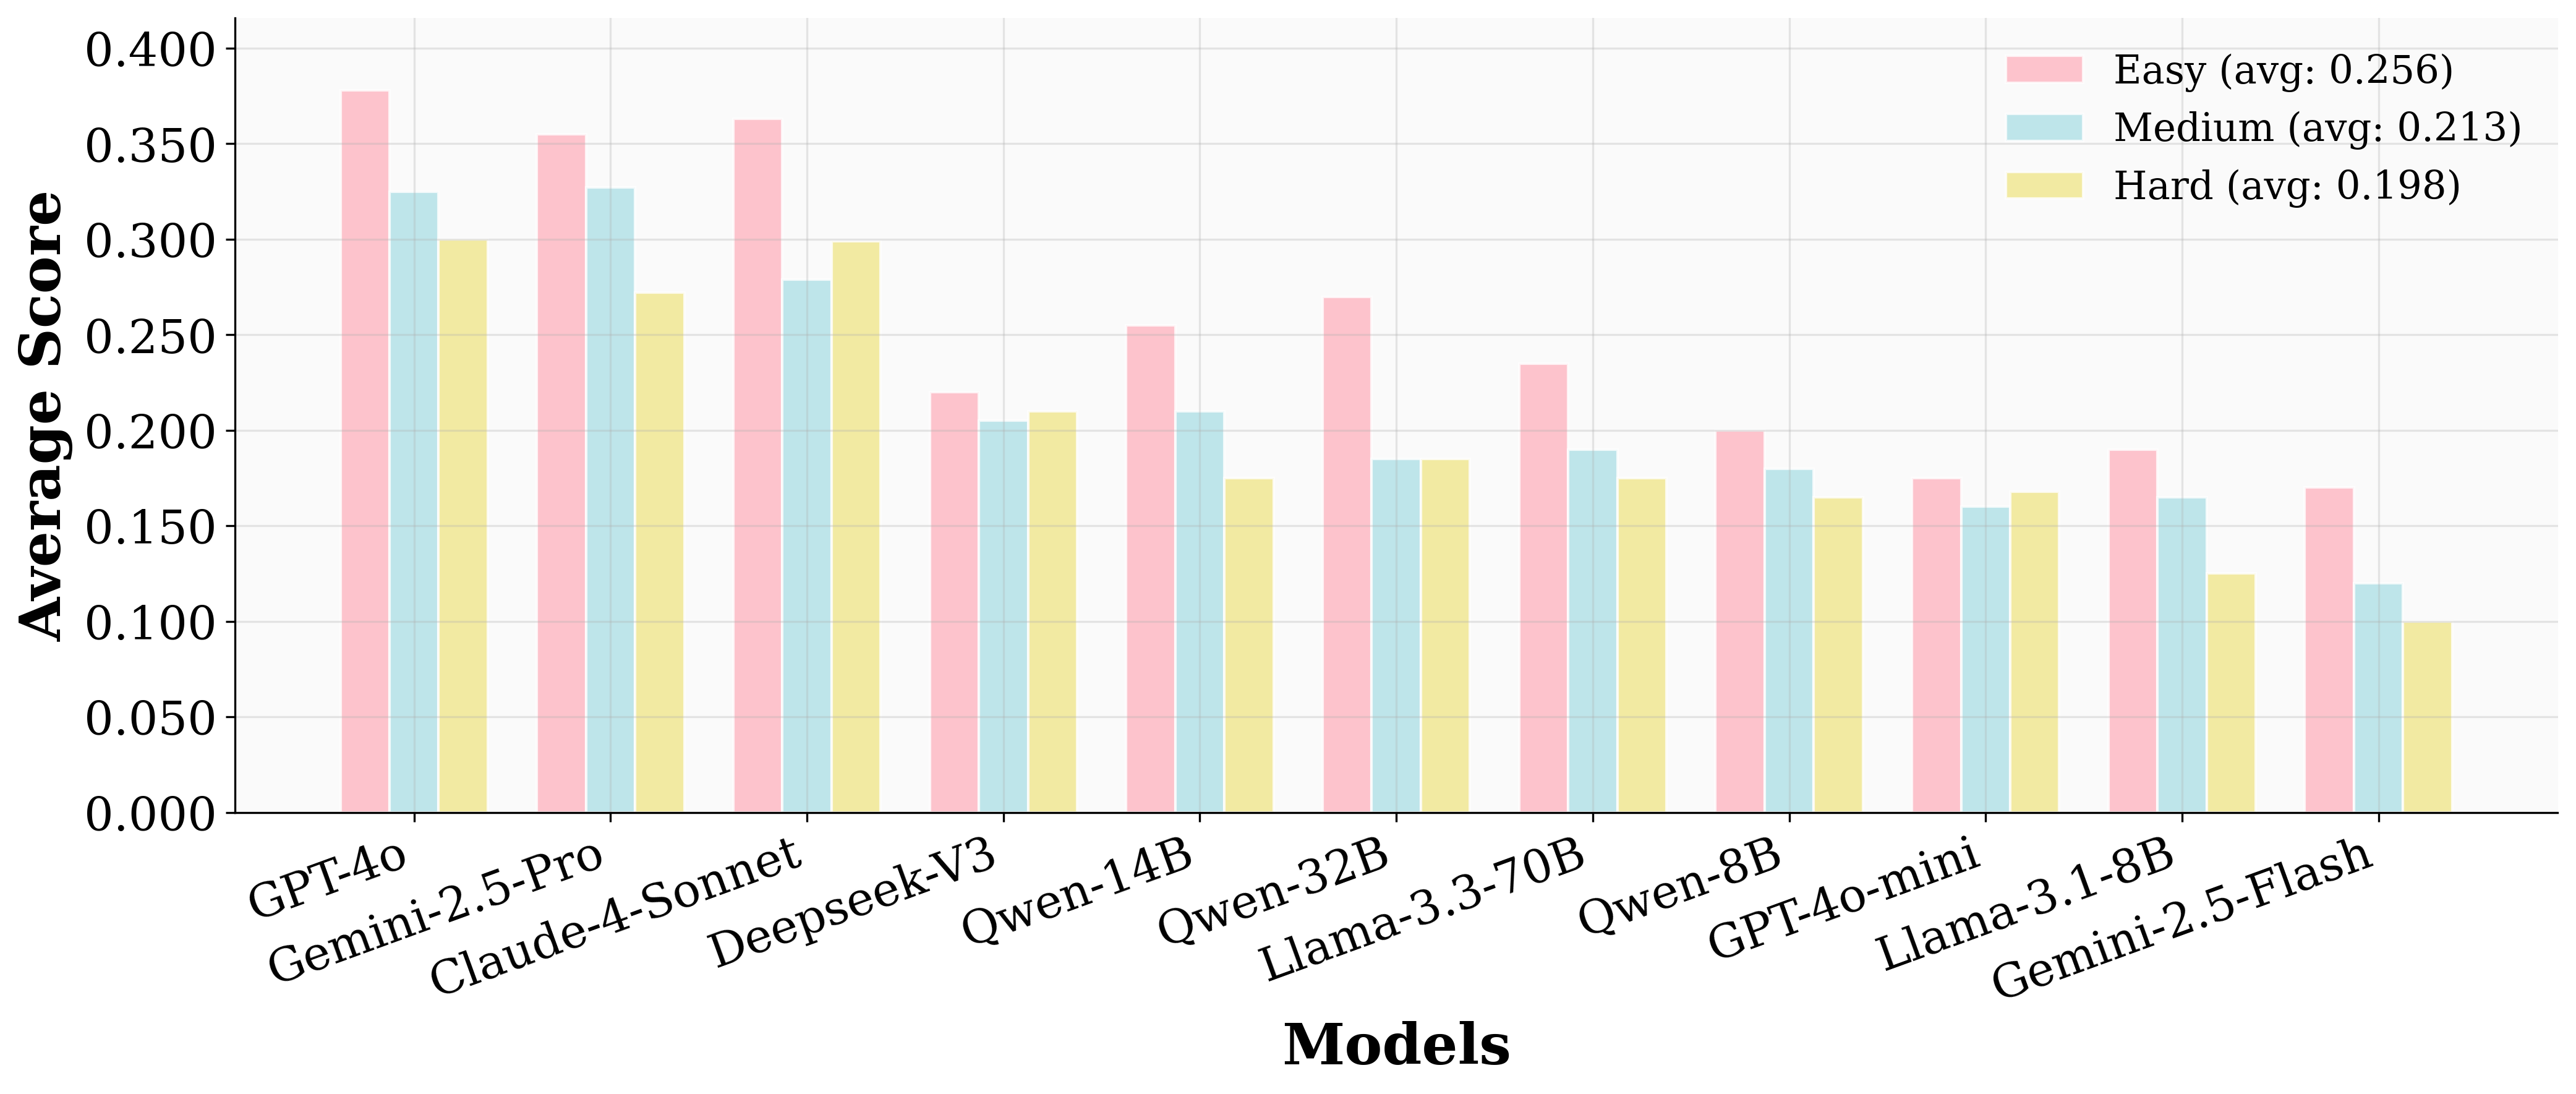
\includegraphics[width=\linewidth]{figures/difficulty_impact.png}
    \end{minipage}
 
    \caption{The score distribution of tested models across three difficulty tiers.}
    \label{fig:difficulty}
    
    \vspace{0pt}
\end{figure}


\paragraph{Difficulty tier division effectively reflects {\gymname}'s challenges.}  
We begin by analyzing how scenario difficulty impacts model performance, as shown in~\Cref{fig:difficulty}. Following the tiering in~\Cref{tab:statistics}, we divide test scenarios into Easy, Medium, and Hard based on preference complexity. Results show a general downward trend in scores as difficulty increases. This confirms that our difficulty stratification captures real reasoning challenges for models. Furthermore, the performance drop within each model across tiers reveals a lack of robustness in managing complex user interactions, which is something humans typically excel at.


\begin{figure}[!t]
    \centering
    \begin{minipage}{1.0\linewidth}
        \centering
        \vspace{0pt}
        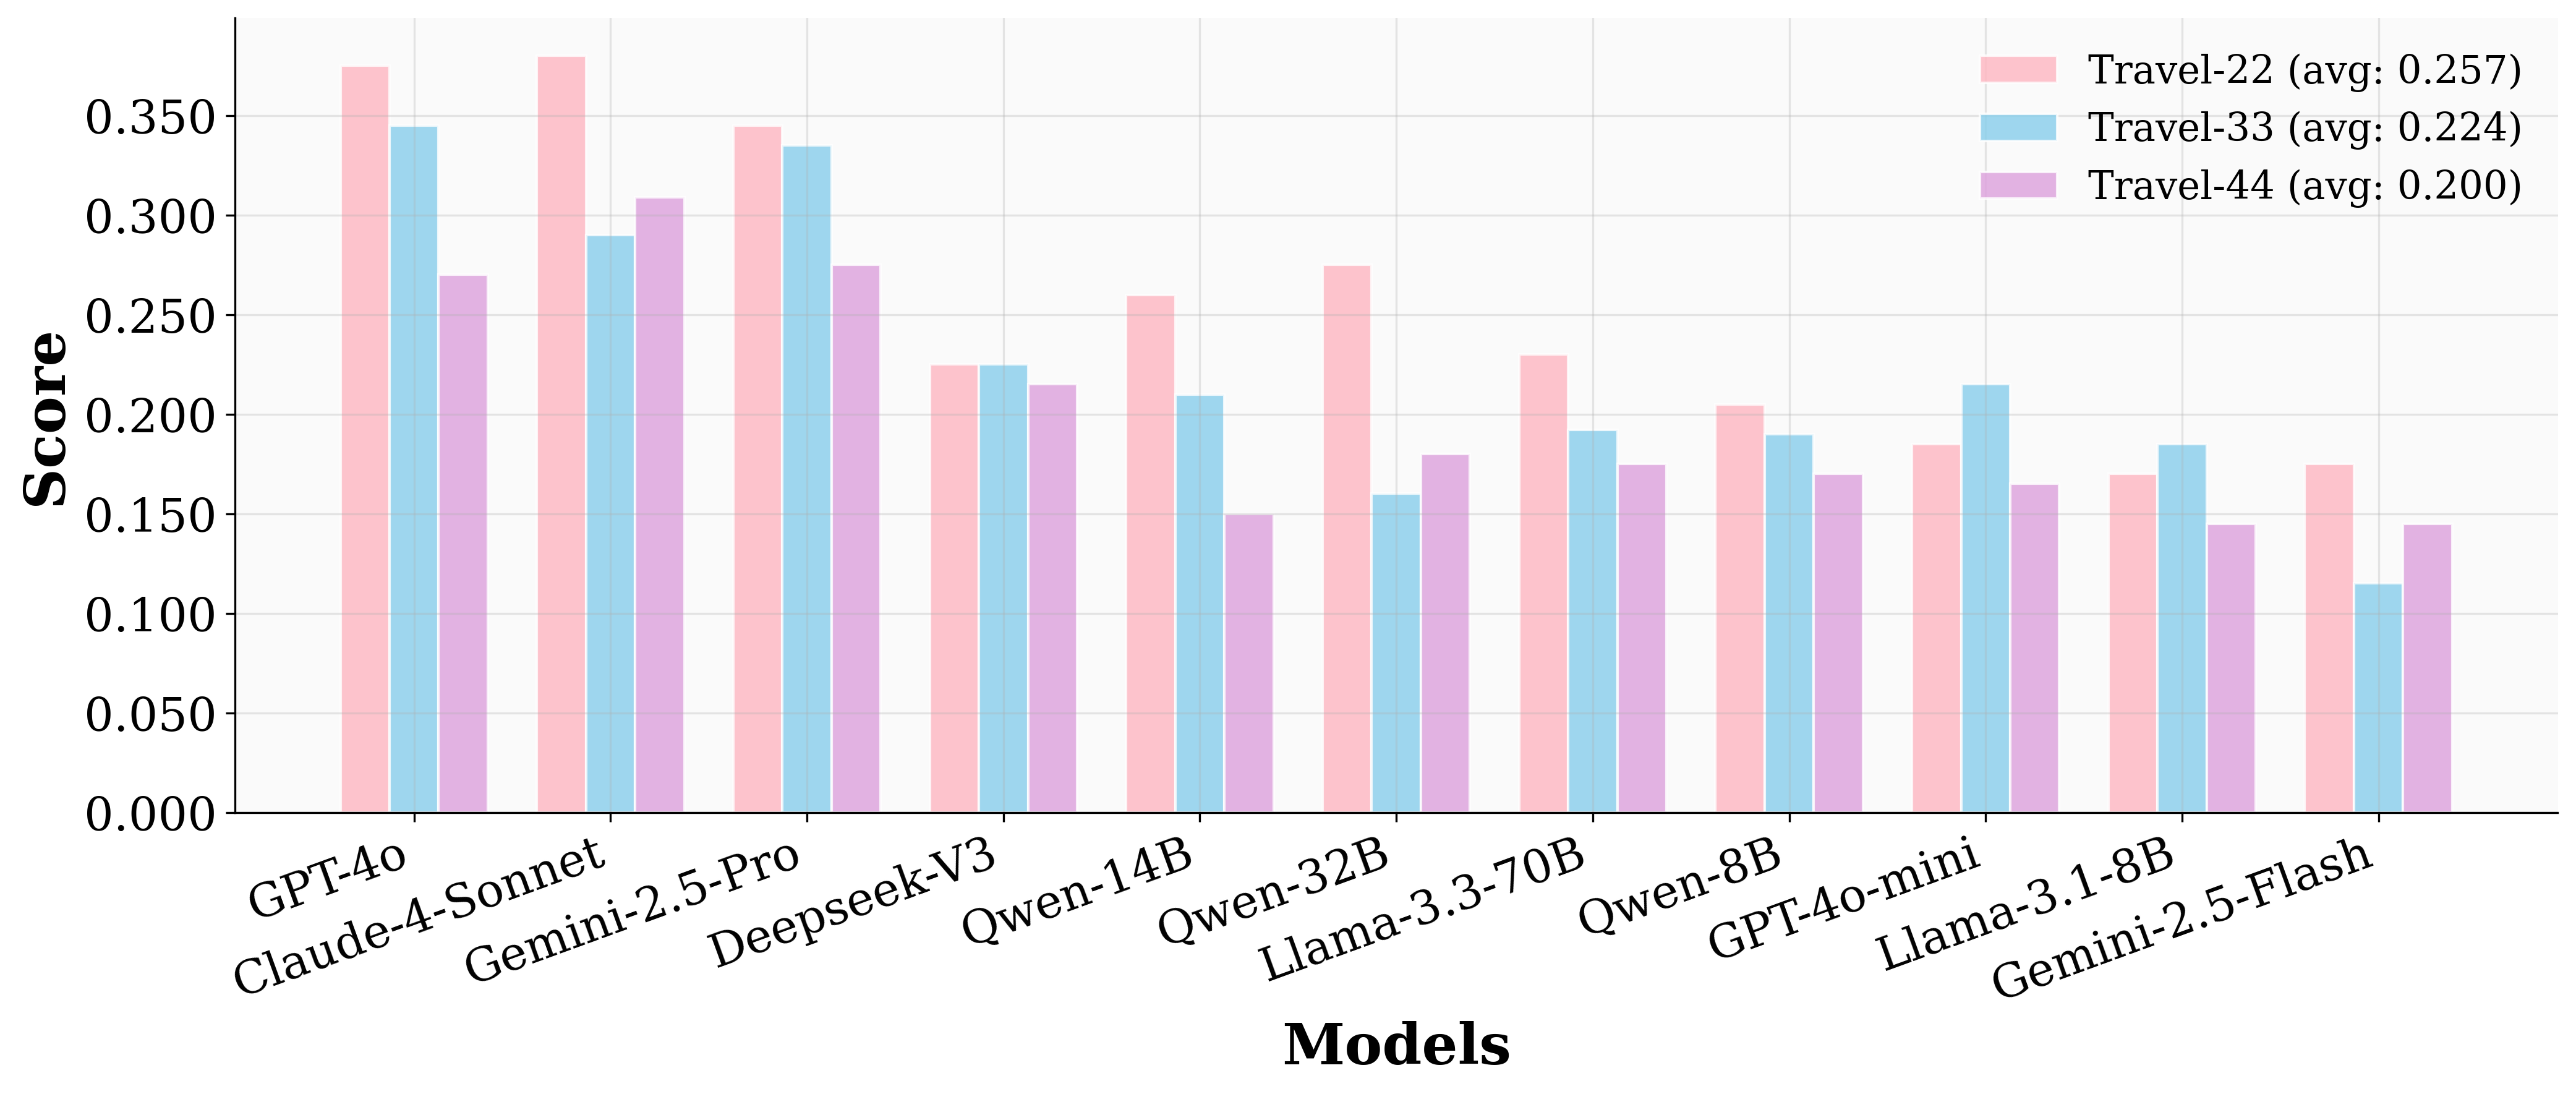
\includegraphics[width=\linewidth]{figures/preference_group1_analysis.png}
    \end{minipage}

    \vspace{2pt}
    
    \begin{minipage}{1.0\linewidth}
        \centering
        \vspace{0pt}
        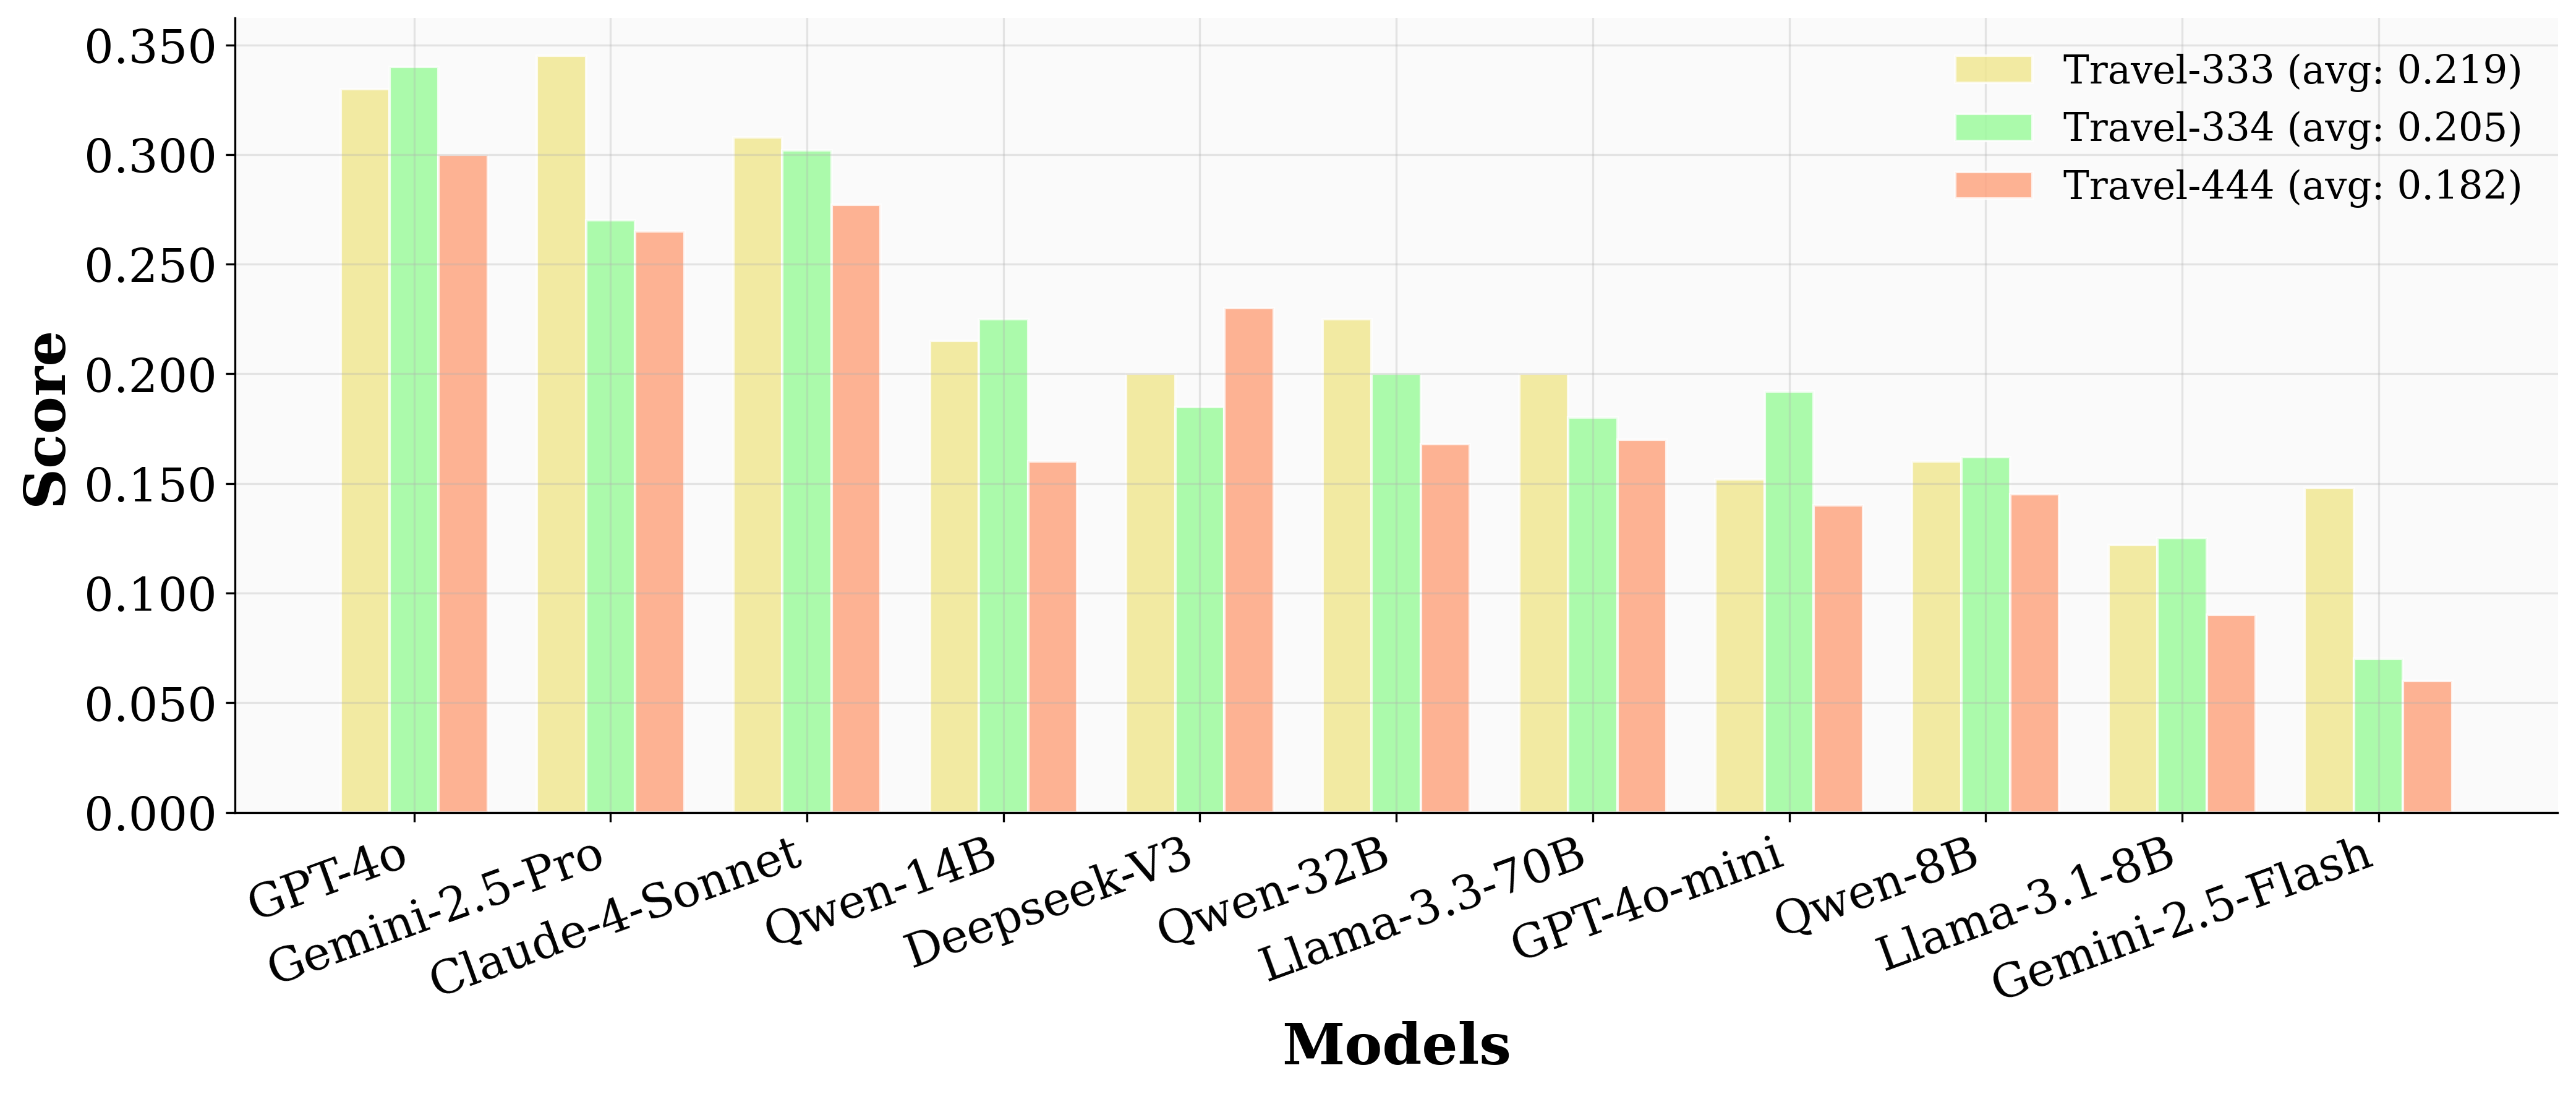
\includegraphics[width=\linewidth]{figures/preference_group2_analysis.png}
    \end{minipage}
    
    \caption{When aspect number is settled, more user preferences generally lead to less scores.}
    \label{fig:preference}
    
    \vspace{0pt}
\end{figure}


\begin{figure}[!t]
    \centering
    \begin{minipage}{1.0\linewidth}
        \centering
        \vspace{0pt}
        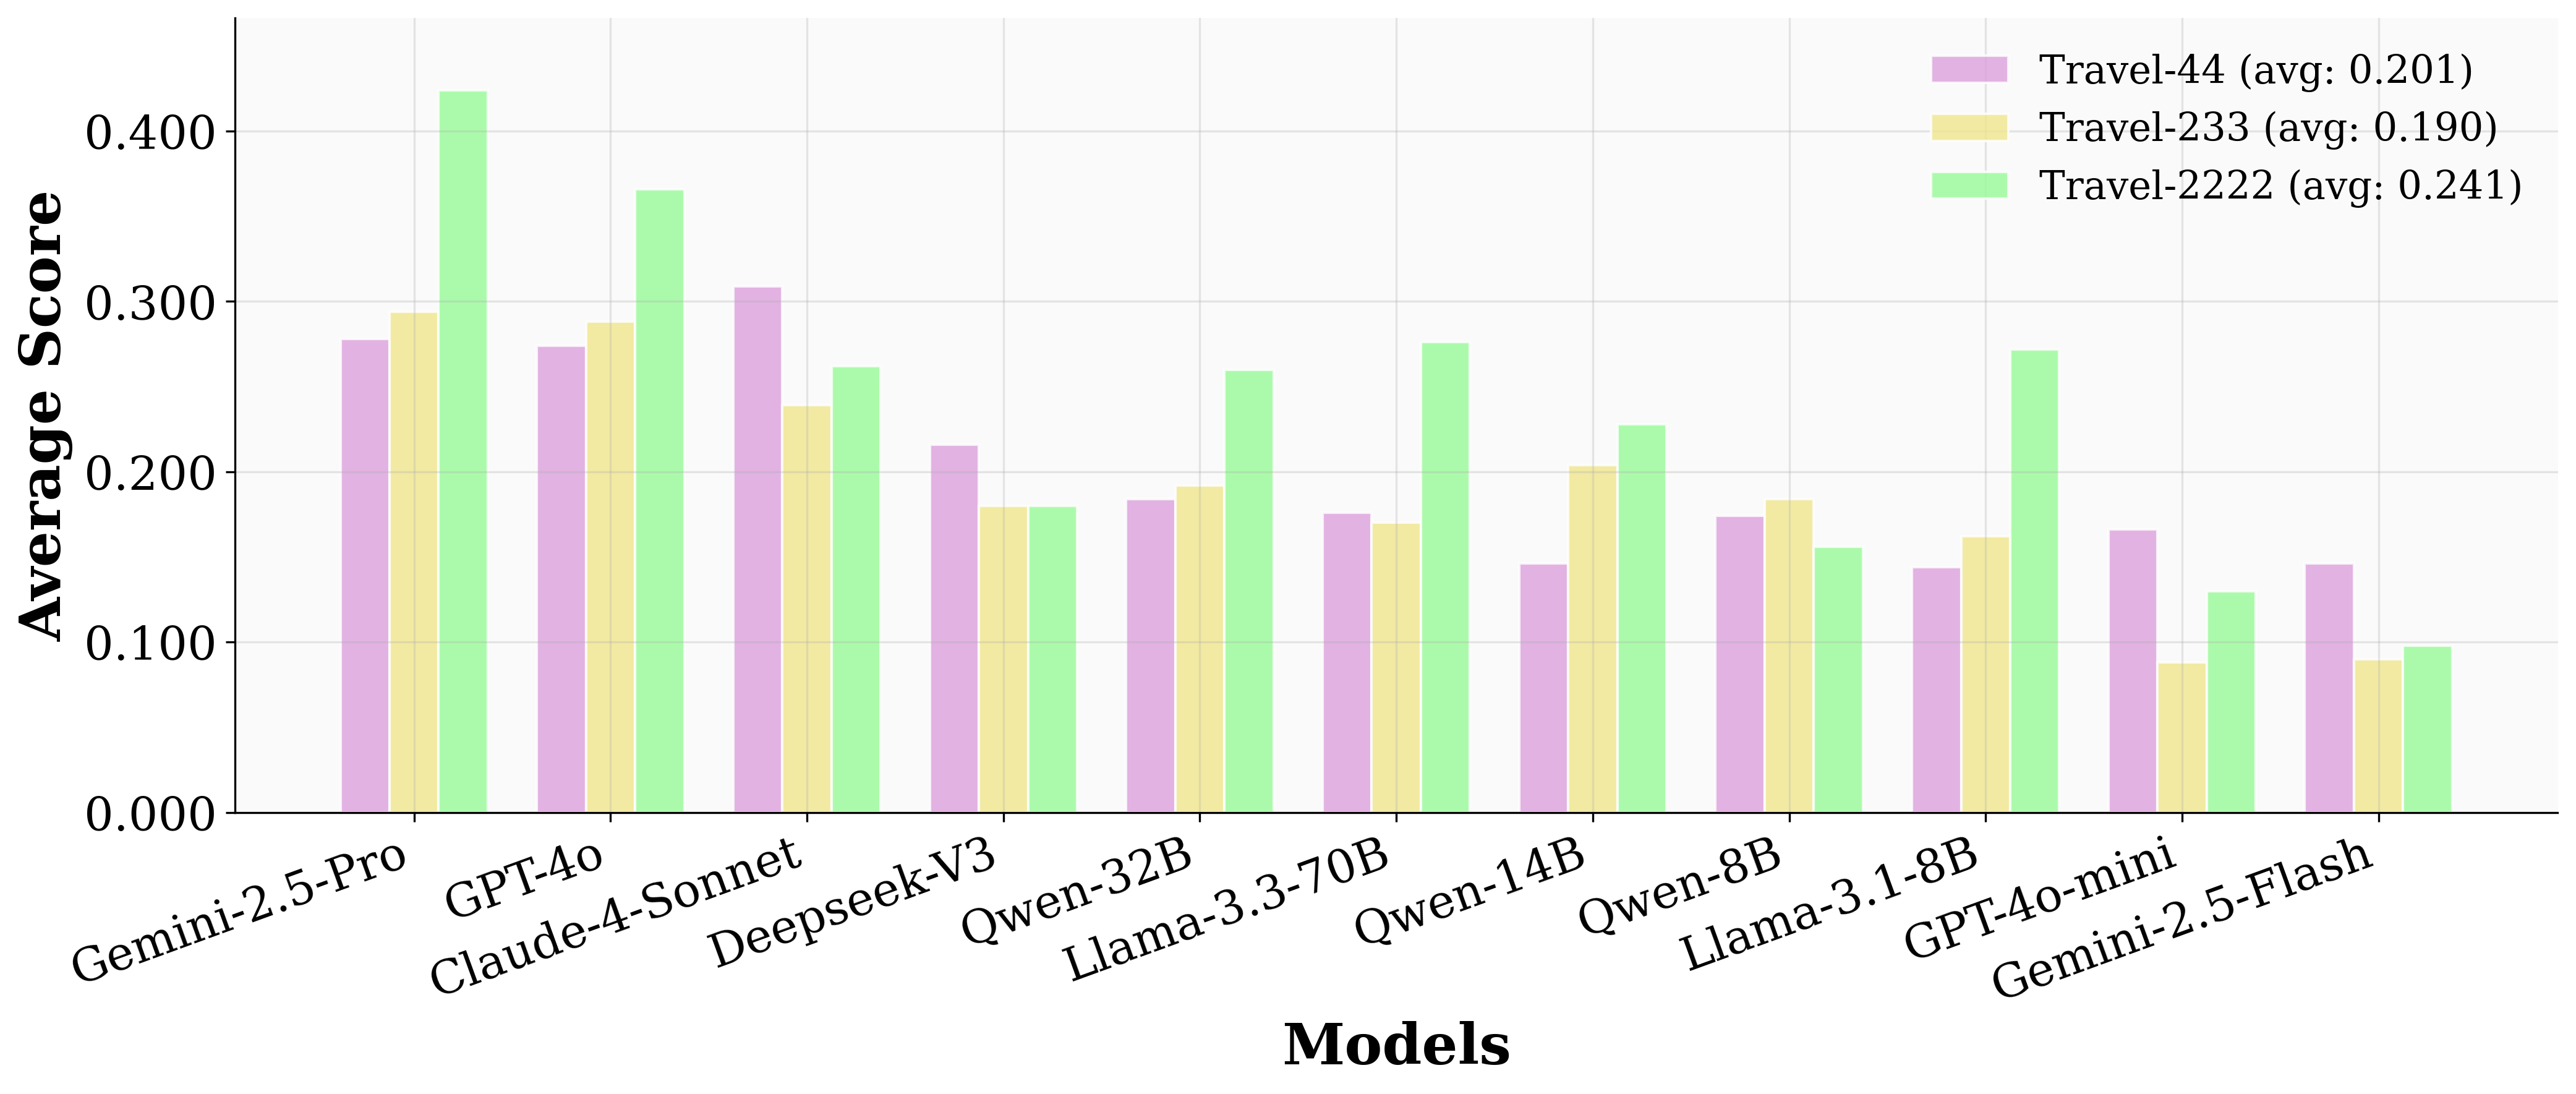
\includegraphics[width=\linewidth]{figures/aspect_impact.png}
    \end{minipage}
 
    \caption{When total user preferences are settled, less preferences per aspect generally lead to higher scores.}
    \label{fig:aspect}
    
    \vspace{0pt}
\end{figure}


\paragraph{The key challenge lies in the number of preferences per aspect.}
To identify the core source of difficulty in {\gymname}, we investigate whether performance is more affected by the number of travel aspects or the number of preferences per aspect. We first fix the number of aspects and vary the number of preferences per aspect. As shown in~\Cref{fig:preference}, model scores consistently decline as the number of preferences increases. This suggests that handling richer user preference signals is a major challenge for current models.

Next, we fix the total number of preferences in a scenario and vary how they are distributed across aspects. As shown in~\Cref{fig:aspect}, performance improves when preferences are more evenly spread across multiple aspects, rather than concentrated within a few. This implies that models reason more effectively when each aspect involves fewer, simpler preferences. Concentrating multiple preferences into a single aspect appears to overload the model’s local reasoning process. Together, these results suggest that the number of preferences per aspect is the main driver of difficulty in {\gymname}.


\begin{table}[!t]
\begin{center}
\small
\tabcolsep=0.005\linewidth
\resizebox{\linewidth}{!}{
\begin{tabular}{lccc}
\toprule
\textbf{Model Name} & \textbf{\makecell{First Index$^{\downarrow}$}} & \textbf{\makecell{Weighted Score$^{\uparrow}$}} & \textbf{\makecell{Correct Exists Rate$^{\uparrow}$}} \\
\midrule
GPT-4o & 3.846 & \textbf{0.054} & \textbf{0.361} \\
Gemini-2.5-Pro & 4.476 & 0.044 & 0.328 \\
Qwen3-8B & 2.005 & 0.039 & 0.186 \\
Qwen3-32B & 2.739 & 0.039 & 0.211 \\
Claude-4-Sonnet & 5.018 & 0.038 & 0.318 \\
Deepseek-V3 & 2.740 & 0.037 & 0.218 \\
Qwen3-14B & 2.650 & 0.035 & 0.197 \\
Llama-3.3-70B & 2.776 & 0.032 & 0.209 \\
Llama-3.1-8B & 1.884 & 0.028 & 0.171 \\
GPT-4o-mini & 2.185 & 0.028 & 0.173 \\
Gemini-2.5-Flash & \textbf{0.927} & 0.014 & 0.080 \\
\bottomrule
\end{tabular}
}
\end{center}
\vspace{-3mm}
\caption{\textbf{Weighted Timing Analysis}: Models evaluated by timing of highest scores and coverage. Weight function $w(i) = 1/(i+1)$ penalizes later discoveries of correct or best user-aligned answer options. Coverage is the micro-average of aspects with valid answers.}
\label{tab:weighted_timing_analysis}
\end{table}

\paragraph{Models struggle to provide answers that are both correct and timely.}
To assess not only whether models find correct or best answers, but also \textit{when} they do so, we conduct a weighted timing analysis in \Cref{tab:weighted_timing_analysis}. Using a weight function $w(i) = 1/(i+1)$, we penalize delayed discoveries, where $i$ is the turn at which a valid answer (reward > 0) first appears. Notably, open-source Qwen models outperform Deepseek in timing, despite Deepseek ranking higher in overall accuracy in~\Cref{tab:travelgym_results_onechoice}. This suggests that while Deepseek eventually finds good answers, it is less efficient in doing so. In contrast, GPT-4o and Gemini-2.5-Pro balance both coverage and timing better, achieving higher Correct Exist Rates and also Weighted Score overall.

We also report the average turn index at which a valid answer first appears. Smaller models, like Llama-3.1-8B and Gemini-2.5-Flash, show lower average indices, indicating the successful attempts of their earlier guesses. However, these guesses often fail, leading to lower Weighted Scores and limited Correct Exist Rates. This reveals a common failure mode: smaller models rely on shallow heuristics or early guesses rather than deeply engaging with user intent. While this may occasionally yield fast correct answers, it more often results in low-quality answers not aligned with user needs.

These findings also help explain the low Preference Elicited in~\Cref{tab:travelgym_results_onechoice} and~\Cref{tab:travelgym_results_multichoice}. Ultimately, a delicate trade-off emerges: models are expected to be efficient in interaction, yet still they should invest enough turns in interaction to truly understand the user's evolving needs or preferences.


\begin{figure}[!t]
    \centering
    \begin{minipage}{1.0\linewidth}
        \centering
        \vspace{0pt}
        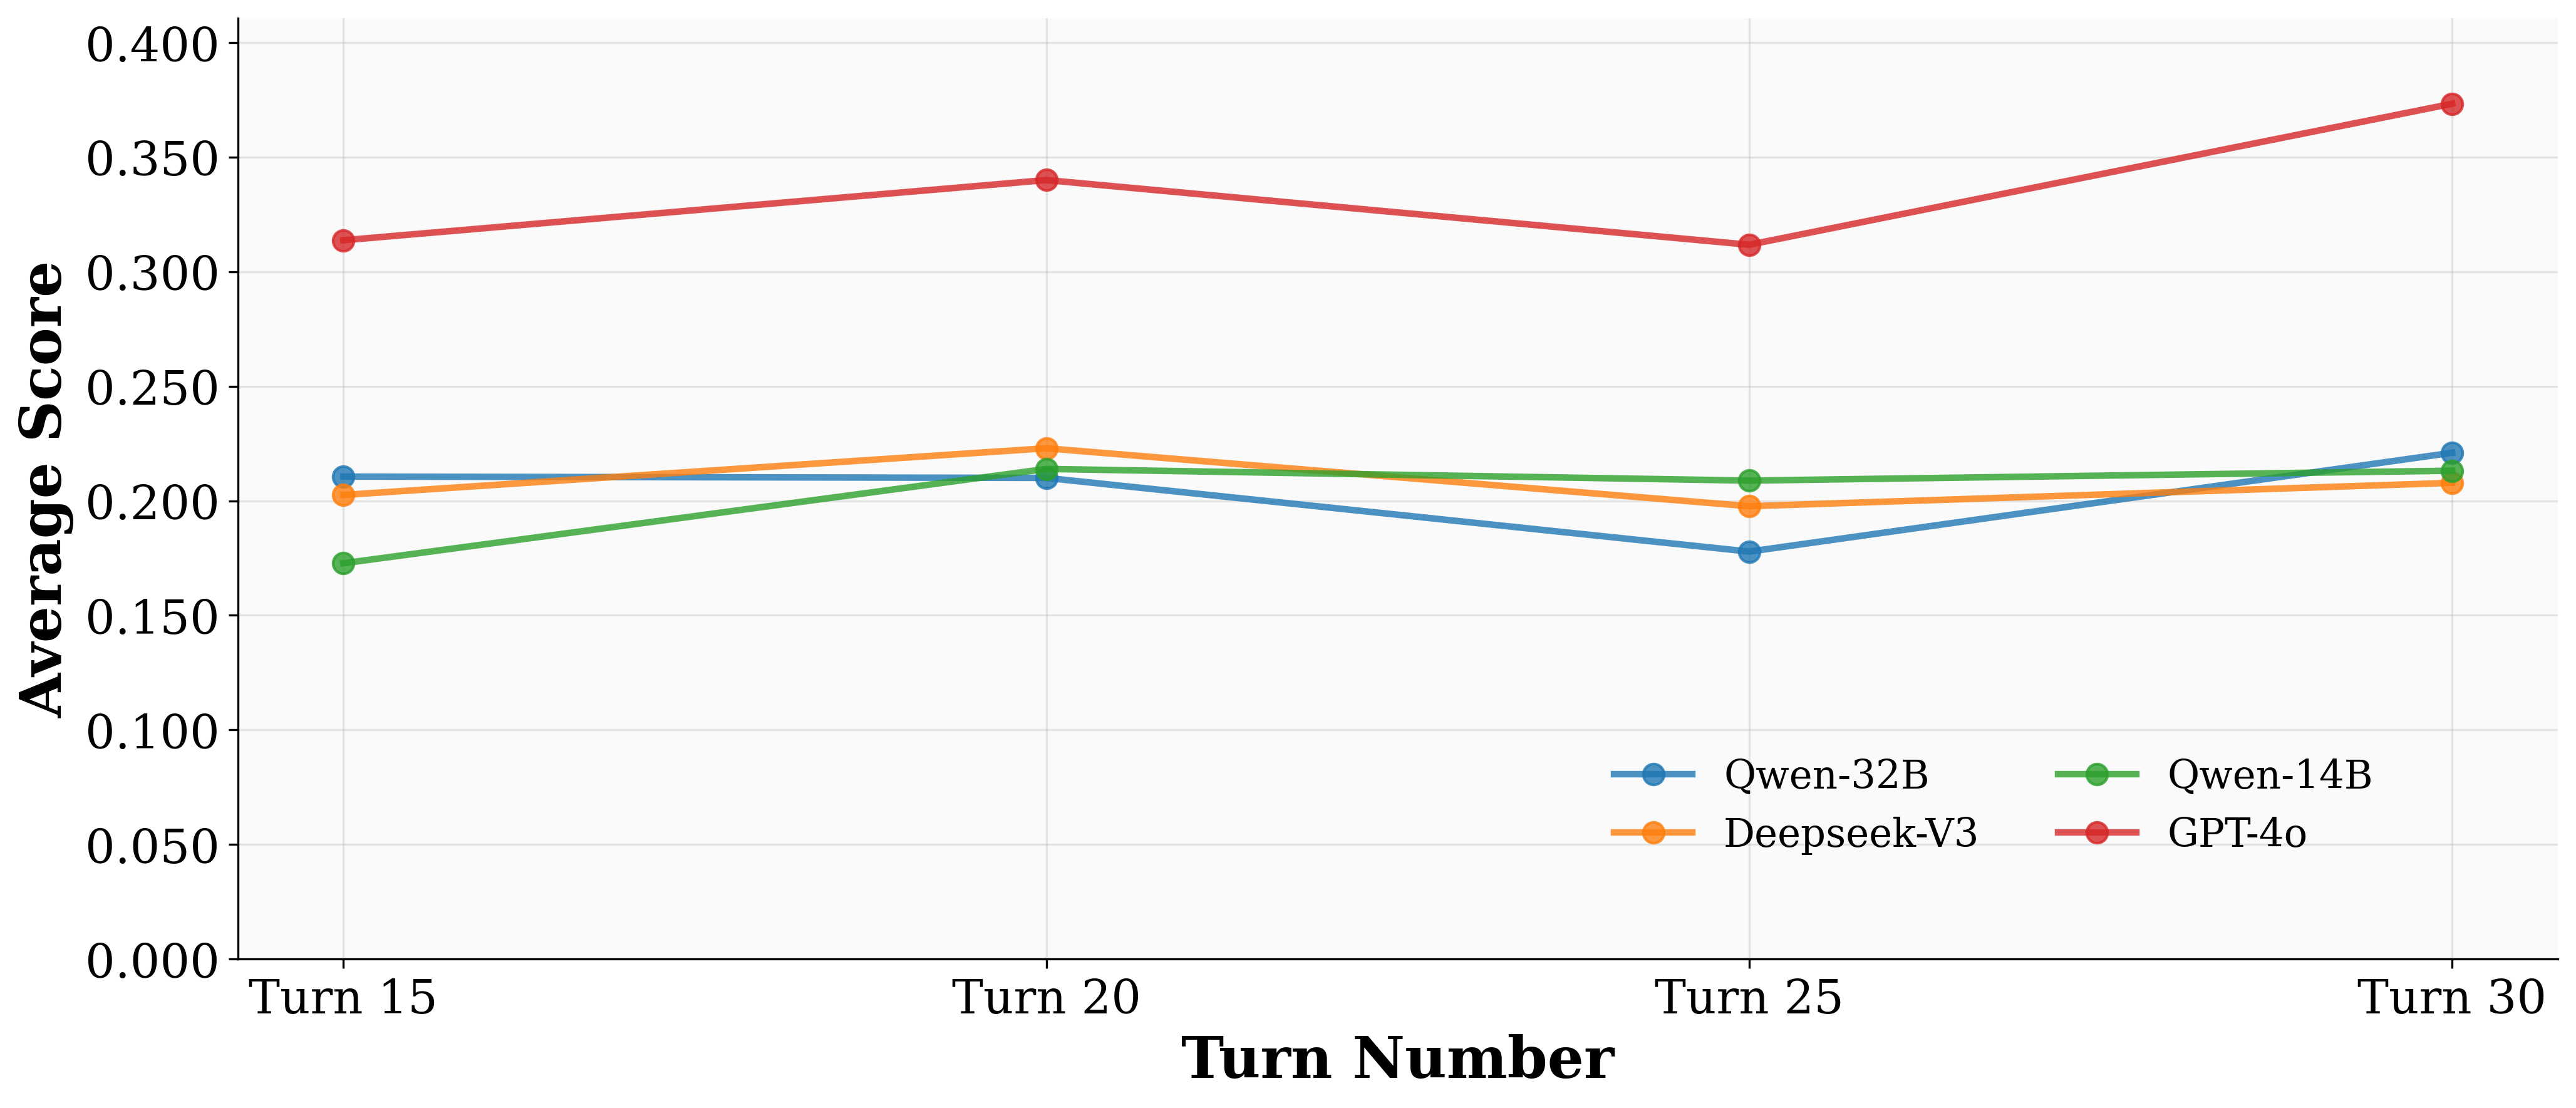
\includegraphics[width=\linewidth]{figures/turn_analysis.png}
    \end{minipage}
 
    \caption{Increasing the number of turns allowed in interaction does not necessarily lead to better performance across models.}
    \label{fig:turn}
    
    \vspace{0pt}
\end{figure}


\paragraph{More interaction turns do not guarantee better performance.}  
We also examine whether increasing the number of interaction turns improves performance, as illustrated in~\Cref{fig:turn}. Surprisingly, simply allowing more turns does not lead to consistent gains, and in some cases, performance even degrades. This suggests that many models fail to leverage the extended interaction window to elicit preferences or refine understanding. Instead, longer conversations often result in repetitive or off-topic dialogue. Without strong dialogue planning and goal-tracking, more turns alone are insufficient to improve performance.


\begin{figure}[!t]
    \centering
    \begin{minipage}{1.0\linewidth}
        \centering
        \vspace{0pt}
        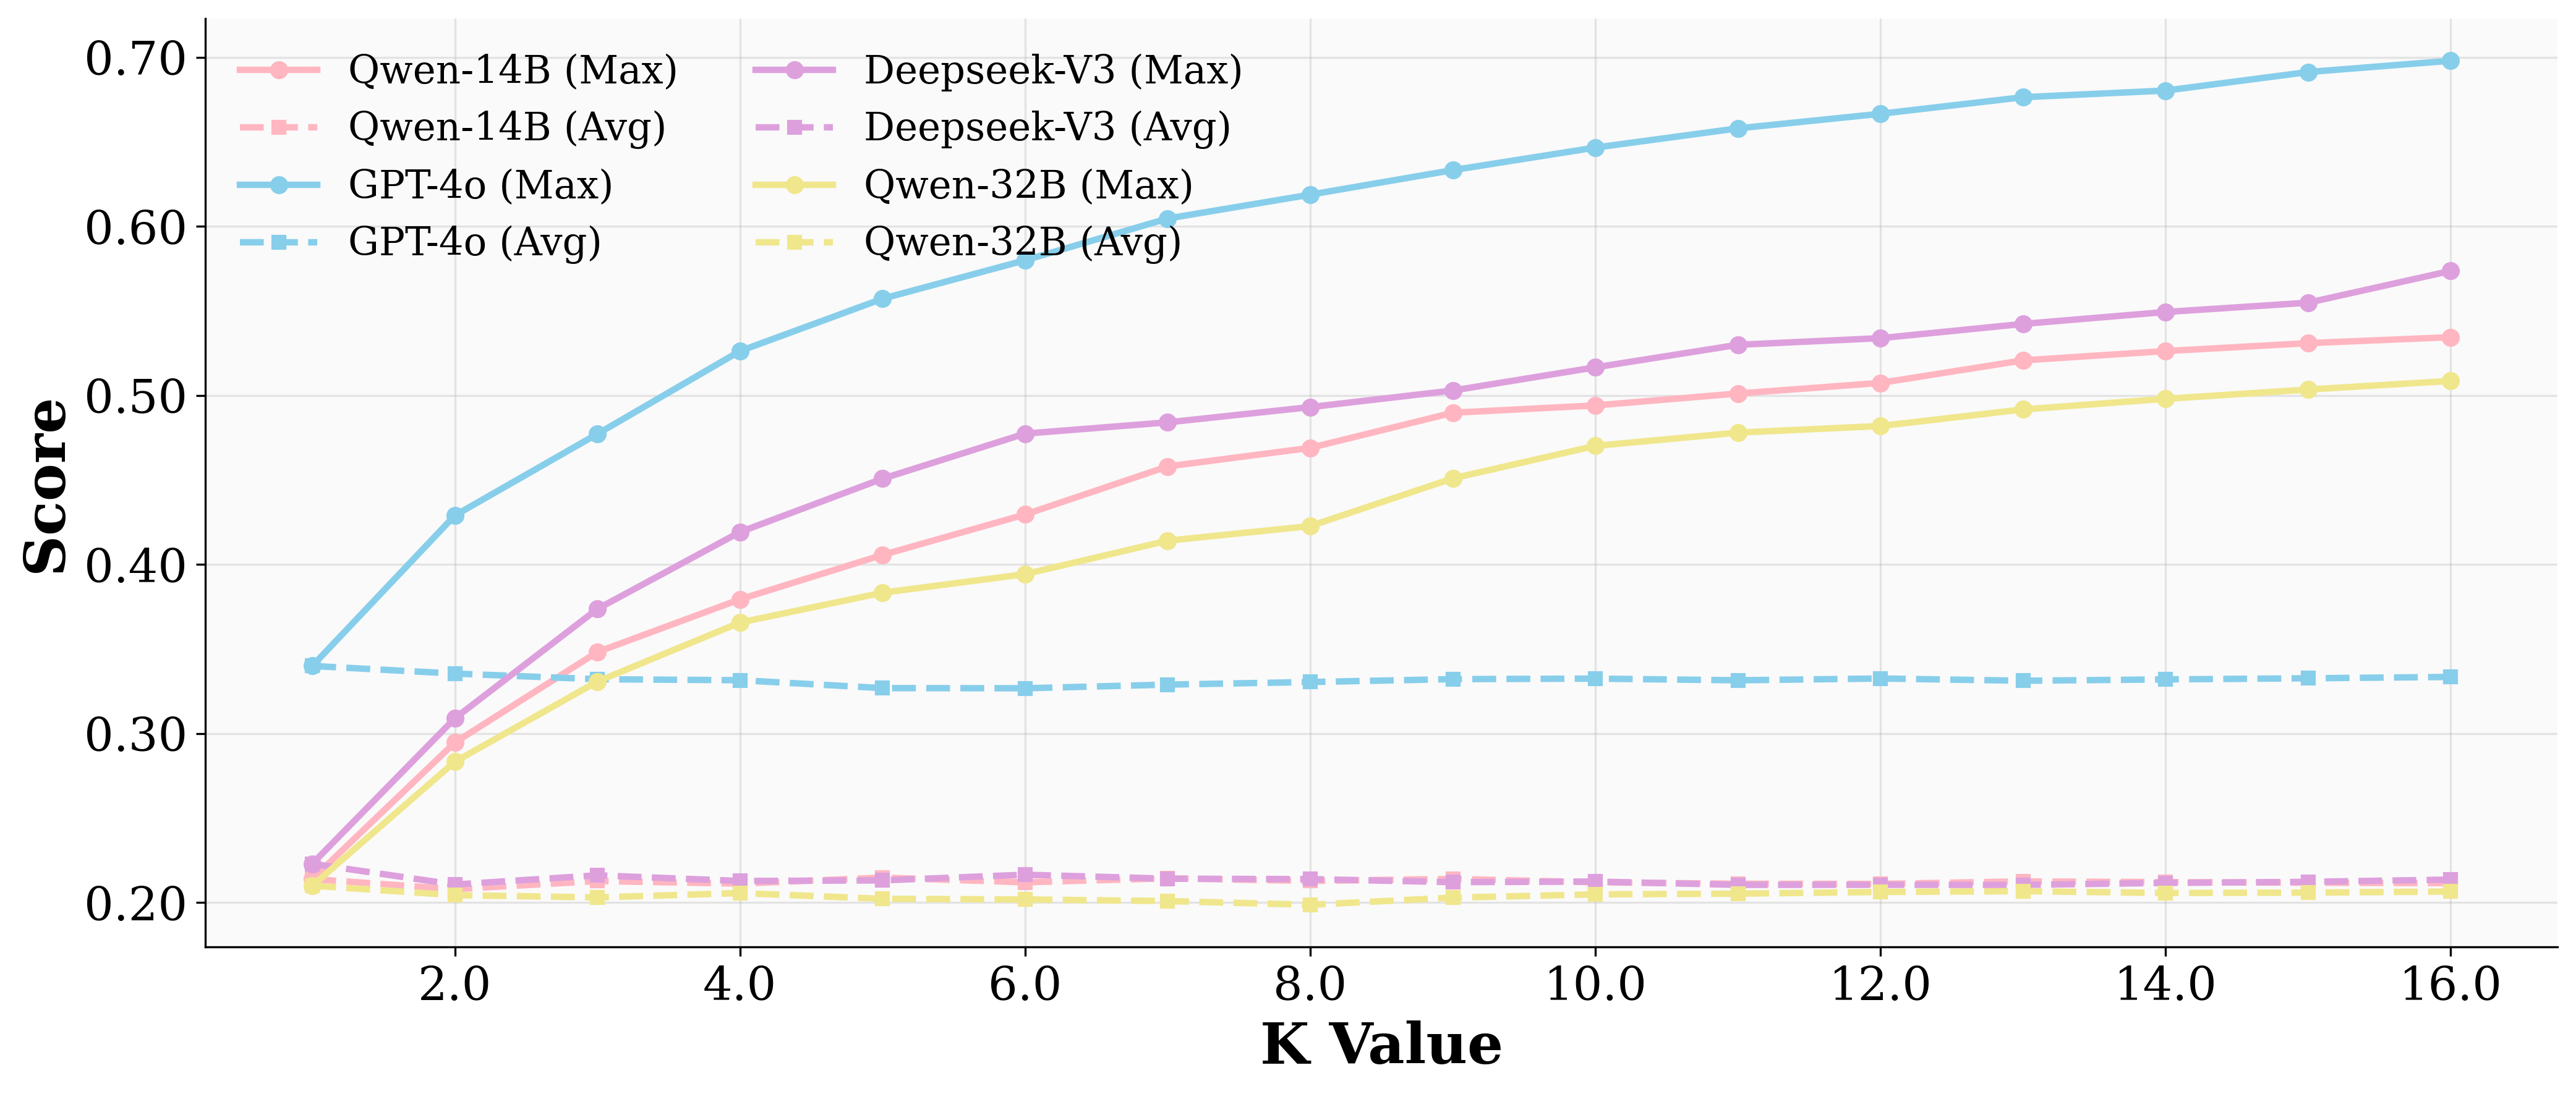
\includegraphics[width=\linewidth]{figures/passk_analysis.png}
    \end{minipage}
 
    \caption{Increasing the number of sampling time raises the maximum score but average score shows little change or even slightly drops.}
    \label{fig:passk}
    
    \vspace{0pt}
\end{figure}


\paragraph{Effect of sampling frequency reveals instability.}  
We analyze the effect of sampling frequency using \textit{pass-$k$} evaluation, as shown in~\Cref{fig:passk}. While the maximum score across $k$ samples steadily increases, the average score remains flat or even declines. This suggests that more samples increase the chance of stumbling upon a good response, but most outputs remain poor. The results highlight a key limitation: current models rely heavily on sampling luck rather than robust reasoning to align with user preferences. Given the high cost of pass-$k$ sampling, this instability poses a challenge for deploying reliable user-interactive systems.


\begin{table}[!t]
\begin{center}
\small
\tabcolsep=0.02\linewidth
\resizebox{1.0\linewidth}{!}{
\begin{tabular}{lcccc}
\toprule
\textbf{Model Name} & \textbf{Original (w10n5)} & \textbf{w10n0} & \textbf{w5n5} & \textbf{w8n2} \\
\midrule
GPT-4o & 0.340 & $0.344_{\green{\uparrow 0.004}}$ & $0.360_{\green{\uparrow 0.020}}$ & $0.350_{\green{\uparrow 0.010}}$ \\
Deepseek-V3 & 0.223 & $0.271_{\green{\uparrow 0.048}}$ & $0.249_{\green{\uparrow 0.027}}$ & $0.241_{\green{\uparrow 0.018}}$ \\
Qwen3-32B & 0.210 & $0.220_{\green{\uparrow 0.010}}$ & $0.241_{\green{\uparrow 0.031}}$ & $0.224_{\green{\uparrow 0.014}}$ \\
Qwen3-14B & 0.214 & $0.225_{\green{\uparrow 0.011}}$ & $0.199_{\red{\downarrow 0.015}}$ & $0.203_{\red{\downarrow 0.011}}$ \\
\bottomrule
\end{tabular}
}
\end{center}
\vspace{-3mm}
\caption{Impact of choice distribution on model scores. ``w10n5'' indicates a setting where, in addition to the correct and best options, there are 10 wrong and 5 noise options as distractors. Each cell reports the model's score and its change relative to the original setup.}
\label{tab:choice}
\end{table}

\paragraph{Less options reduces interference but do not reduce the core challenge.} 
We finally perform an ablation study to assess how the number of wrong and noise options affects model performance. As shown in~\Cref{tab:choice}, reducing these distractors generally improves scores. However, even for strong models like Deepseek-V3 and GPT-4o, removing five wrong or noise options (about 30\% of the total) yields only modest gains. Interestingly, some smaller models, such as Qwen-14B, even show slight performance drops. These results suggest that (1) reducing options does not fundamentally lower task difficulty: fully understanding user preferences remains essential, as only one best option satisfies all constraints (budget constraint included); and (2) many models still rely on shallow guessing rather than genuine preference understanding, which limits their ability to benefit from reduced distractors. These results also indirectly highlights the intentional complexity designed into our option sets for each data scenario.
